\usetikzlibrary{arrows.meta,calc,shapes.geometric}
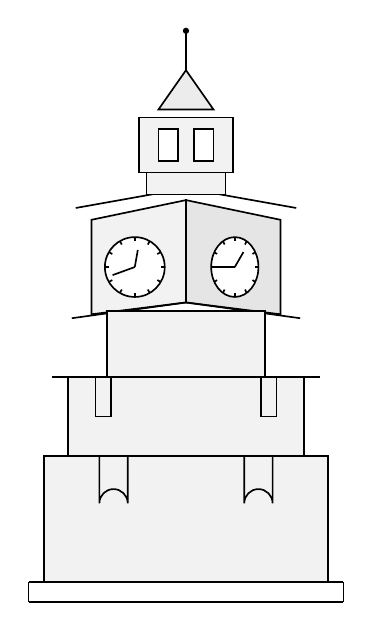
\begin{tikzpicture}[x=1cm,y=1cm,line width=.6pt,font=\normalsize]
\coordinate (SP1) at (0.0,7.0);
\coordinate (SP0) at (0.0,6.0);
\coordinate (BE1) at (-0.6,5.9);
\coordinate (BE2) at (0.6,5.9);
\coordinate (BE0) at (-0.6,5.2);
\coordinate (BE3) at (0.6,5.2);
\coordinate (CF1) at (-1.2,4.6);
\coordinate (CF2) at (0.0,4.85);
\coordinate (CF3) at (1.2,4.6);
\coordinate (CF0) at (-1.2,3.4);
\coordinate (CF3b) at (1.2,3.4);
\coordinate (CKF) at (-0.65,4.0);
\coordinate (CKS) at (0.62,4.0);
\coordinate (LW0) at (-1.8,0.0);
\coordinate (LW1) at (1.8,0.0);
% spire + finial
\draw (SP0) -- (SP1);
\filldraw[fill=gray!15] (SP0) -- (-0.35,6.0) -- (0.0,6.5) -- (0.35,6.0) -- cycle;
\fill (SP1) circle (0.04);
% belfry
\filldraw[fill=gray!10] (BE0) -- (BE1) -- (BE2) -- (BE3) -- cycle;
\filldraw[fill=white] (-0.35,5.35) rectangle (-0.1,5.75);
\filldraw[fill=white] (0.1,5.35) rectangle (0.35,5.75);
% clock stage: front face + side face sharing corner edge
\filldraw[fill=gray!10] (CF0) -- (CF1) -- (CF2) -- (0.0,3.55) -- cycle;
\filldraw[fill=gray!20] (0.0,3.55) -- (CF2) -- (CF3) -- (CF3b) -- cycle;
\draw (0.0,3.55) -- (CF2);
% roof rims
\draw[line width=.6pt] (-1.45,3.35) -- (0.0,3.55) -- (1.45,3.35);
\draw[line width=.6pt] (-1.4,4.75) -- (0.0,5.0) -- (1.4,4.75);
% clocks: front circle, side ellipse (adjacent-face perspective)
\draw[fill=white] (CKF) circle (0.38);
\draw[fill=white] (CKS) ellipse (0.30 and 0.38);
\foreach \a in {0,30,...,330} {
  \draw ($(CKF)+(\a:0.33)$) -- ($(CKF)+(\a:0.38)$);
}
\foreach \a in {0,30,...,330} {
  \draw ($(CKS)+(\a:0.26 and 0.33)$) -- ($(CKS)+(\a:0.30 and 0.38)$);
}
% schematic hands (not claiming photo times)
\draw (CKF) -- ++(80:0.22);
\draw (CKF) -- ++(200:0.30);
\draw (CKS) -- ++(60:0.22);
\draw (CKS) -- ++(180:0.28);
% connector shaft: clock stage to mid body (staged tower, no floating gap)
\filldraw[fill=gray!10] (-1.0,2.6) -- (-1.0,3.44) -- (1.0,3.44) -- (1.0,2.6) -- cycle;
% connector neck: belfry to clock-stage roof
\filldraw[fill=gray!10] (-0.5,4.92) -- (-0.5,5.2) -- (0.5,5.2) -- (0.5,4.92) -- cycle;
% mid + lower staged bodies
\filldraw[fill=gray!10] (-1.5,2.6) -- (1.5,2.6) -- (1.5,1.6) -- (-1.5,1.6) -- cycle;
\draw[line width=.6pt] (-1.7,2.6) -- (1.7,2.6);
\draw[line width=.6pt] (-1.7,1.6) -- (1.7,1.6);
\filldraw[fill=gray!10] (-1.8,0.0) -- (-1.8,1.6) -- (1.8,1.6) -- (1.8,0.0) -- cycle;
% arched openings
\draw (-1.1,1.6) -- (-1.1,1.0) arc (180:0:0.18) -- (-0.74,1.6);
\draw (0.74,1.6) -- (0.74,1.0) arc (180:0:0.18) -- (1.1,1.6);
\draw (-1.15,2.6) -- (-1.15,2.1) -- (-0.95,2.1) -- (-0.95,2.6);
\draw (0.95,2.6) -- (0.95,2.1) -- (1.15,2.1) -- (1.15,2.6);
% base steps
\draw (-2.0,0.0) -- (2.0,0.0);
\draw (-2.0,-0.25) -- (2.0,-0.25);
\draw (-2.0,0.0) -- (-2.0,-0.25);
\draw (2.0,0.0) -- (2.0,-0.25);
\end{tikzpicture}
